\section{Prompts}
\label{app:prompts}

\paragraph{Selector.} The \qss{} selector receives the following system instruction, followed by the index (or the prefiltered index) and the question. The output is constrained to the JSON schema \texttt{\{"rounds": [string]\}}.

\begin{quote}\small
You are the retrieval step of a personal assistant's long-term memory. You get a compact index of the user's entire conversation history (one line per round; images are summarised in a few words) and a question. Choose the rounds that must be opened in full (with their original images) to answer the question. Include EVERY round that may hold needed evidence, especially ALL members of any group the question refers to (e.g. all ads of a brand, every scene of an episode, all versions of a screen over time), not just the best match. Include rounds that define labels the question uses (episode/arc names, `first', `later', `updated'). Image summaries are lossy: when unsure whether an image is relevant, include it. Order by importance. Return JSON with the key ``rounds'' and at most 40 ids.
\end{quote}

\paragraph{Controls.} The ranking control receives the same candidate index lines with the instruction to rank all candidate rounds from most to least useful for answering the question and to return all identifiers in order. The recall-oriented ranking control receives the selector instruction above with only its output changed: it ranks all candidates by how likely they must be opened, ranking first every round that may hold needed evidence, all members of any group that the question refers to, rounds that define labels used by the question, and rounds whose image summary is too coarse to rule them out. The graded-relevance control rates every candidate from 0 (not relevant) to 3 (contains needed evidence) and keeps the rounds graded 2 or 3. Selectors from other families receive the identical selector instruction through OpenRouter with JSON output.

\paragraph{Per-member notes.} On the widened path, the note writer (\texttt{gemini-2.5-flash-lite}) reads each selected round with its images and is asked to copy exact numbers, names, labels, and dates, and to return the facts that could be part of the answer, such as one of several items that the question totals, counts, compares, or orders, an earlier or later state of something that the question asks about, or a date needed for a computation. Each fact cites its round identifier, and the reader receives the list of facts under a short header before the raw rounds.

\paragraph{Reader.} All conditions with the same reader share one system instruction. It asks the reader to ground every answer in the provided history and images, to prefer the most recent evidence when information conflicts, to inspect images carefully, to state when information is absent, to name images the way the conversation described them, and to answer concisely. The shared reader prompt includes an example phrase (``the provisional busy-day trend'') that matches the reference answers of two MemEye questions; excluding these questions changes the main differences by at most 0.001.

\paragraph{Judges.} On MemEye, the judge uses the official rubric, which scores an answer in $\{0, 0.25, 0.5, 0.75, 1\}$ against the reference answer. On MemLens, the judge uses the official type-specific prompts of the benchmark (binary scores) without modification.

\section{Text Benchmarks and Multimodal Baselines}
\label{app:text}

Table~\ref{tab:prelim} reports the comparison of Section~\ref{sec:problem}. On LoCoMo and LongMemEval-S, cosine retrieval with a large budget is within one point of full-context reading. On MemEye, full-context reading with low-resolution images is the most accurate input for the strong reader, high resolution adds tokens but no accuracy, and dense captions in place of images lower accuracy. Captions are nevertheless useful as retrieval keys (Figure~\ref{fig:app_keys}a), because relevant images score below unrelated text in the shared embedding space~\citep{liang2022modalitygap}; all experiments therefore index rounds with captions but give readers the original images. Figure~\ref{fig:app_keys}b shows that only the strongest reader benefits from the whole history, whereas lighter readers are most accurate on focused evidence.

\begin{table*}[t]
\centering
\small
\resizebox{\textwidth}{!}{%
\begin{tabular}{llccr}
\toprule
\rowcolor{hHead} Benchmark & Condition & Accuracy & $\Delta$ vs.\ full context & Tokens \\
\midrule
\multirow{3}{*}{LoCoMo (1,540 q)} & Full context & 0.790 & -- & 32,499 \\
 & Cosine top-100 turns & 0.781 & $-0.009$ $[-0.023, +0.006]$ & 5,693 \\
 & Cosine top-10 turns & 0.706 & $-0.084$ $[-0.105, -0.064]$ & 755 \\
\midrule
\multirow{3}{*}{LongMemEval-S (119 q)} & Full context & 0.950 & -- & 113,227 \\
 & Cosine top-50 rounds & 0.941 & $-0.008$ $[-0.034, +0.017]$ & 21,730 \\
 & Cosine top-10 rounds & 0.899 & $-0.050$ $[-0.092, -0.017]$ & 4,986 \\
\midrule
\multirow{7}{*}{MemEye (371 q)} & Full context, images at low resolution & 0.819 & -- & 27,232 \\
 & Full context, images at high resolution & 0.811 & $-0.008$ $[-0.036, +0.020]$ & 78,961 \\
 & Full context, dense captions instead of images & 0.779 & $-0.040$ $[-0.077, -0.005]$ & 55,309 \\
 & Full context, no visual information & 0.191 & -- & 11,262 \\
 & Cosine top-40 rounds, images & 0.741 & $-0.079$ $[-0.112, -0.047]$ & 11,136 \\
 & Cosine top-10 rounds, images & 0.689 & $-0.130$ $[-0.173, -0.090]$ & 3,916 \\
 & Annotated evidence, images & 0.746 & $-0.073$ $[-0.115, -0.034]$ & 2,039 \\
\bottomrule
\end{tabular}}
\caption{\textbf{Raw retrieval versus full-context reading.} $\Delta$ is the paired difference from full context with a 95\% bootstrap interval; tokens are prompt tokens per question. LoCoMo and LongMemEval-S use the strict LongMemEval judge; MemEye uses its official 0--1 rubric. ``Annotated evidence'' reads only the gold evidence rounds.}
\label{tab:prelim}
\end{table*}
\begin{figure*}[t]
\centering
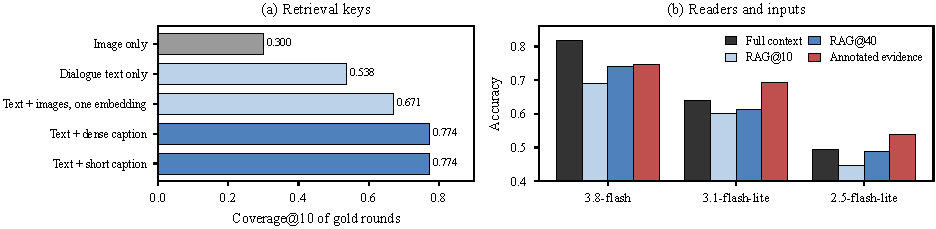
\includegraphics[width=\textwidth]{figures/app_keys_reader.pdf}
\caption{(a)~Retrieval keys on MemEye: fraction of gold evidence rounds among the top 10 (371 questions; \texttt{gemini-embedding-2}). (b)~Accuracy on MemEye by reader and input, with images at the standard resolution of each reader and no thinking for \texttt{gemini-2.5-flash-lite}.}
\label{fig:app_keys}
\end{figure*}
\section{Robustness}
\label{app:robust}

\paragraph{Scenario-level uncertainty.} MemEye has eight scenario histories, so question-level intervals may overstate the effective sample size. Figure~\ref{fig:app_cluster} repeats the main MemEye contrasts under a two-stage bootstrap that resamples scenarios and then questions within them; a Wilcoxon signed-rank test over the eight scenario means gives $p=0.031$ for the strong-reader gain with the index and $p=0.078$ for the lightweight-reader gain. The retrieval gain over cosine retrieval of the same size is positive in all eight scenarios, and the strong-reader gain of set selection with the index as context keeps an interval above zero, whereas the lightweight-reader gain does not.

\begin{figure*}[t]
\centering
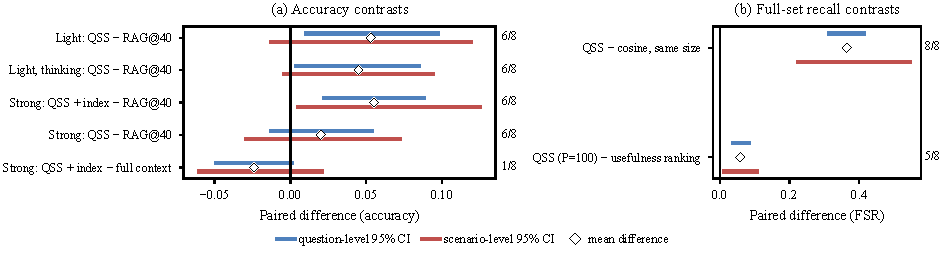
\includegraphics[width=\textwidth]{figures/app_cluster.pdf}
\caption{Question-level and scenario-level 95\% bootstrap intervals for the main MemEye contrasts; the numbers on the right give how many of the eight scenarios have a positive mean difference.}
\label{fig:app_cluster}
\end{figure*}
\paragraph{Independent judge.} Qwen3-VL-235B-A22B re-scored the main MemEye conditions with the same rubric. Its scores are lower than those of the primary judge, exact agreement ranges from 0.69 to 0.87 per condition, and every ordering is preserved: for the lightweight reader, \qss{} 0.514, annotated evidence 0.520, full context 0.469, and RAG@40 0.457; for the strong reader, full context 0.758, \qss{} with index 0.739, \qss{} 0.701, and RAG@40 0.695.

\paragraph{Decoding and selection randomness.} The lightweight reader runs at temperature 0 without thinking; the strong reader varies between seeds by 0.01 to 0.04 on condition means. The strong selector also varies between draws: only about half of the selected sets are identical across two draws on MemEye, and four draws vary the accuracy of the lightweight reader between 0.507 and 0.541.

\paragraph{Independent run.} Table~\ref{tab:rerun} repeats the main contrasts with regenerated image descriptions and new selection draws.

\begin{table}[t]
\centering
\small
\setlength{\tabcolsep}{3.5pt}
\begin{tabular}{l|c|c}
\toprule
\rowcolor{hHead} \textbf{\vgs{} $-$ RAG@40} & \textbf{Main run} & \textbf{Independent run} \\
\midrule
MemEye, light & $+0.053$ $[+0.009, +0.098]$ & $+0.017$ $[-0.023, +0.057]$ \\
MemEye, strong & $+0.048$ $[+0.015, +0.082]$ & $+0.053$ $[+0.018, +0.090]$ \\
VisualMem, light & $+0.115$ $[+0.075, +0.157]$ & $+0.151$ $[+0.111, +0.191]$ \\
\bottomrule
\end{tabular}
\caption{\textbf{Main and independent runs.} Paired differences with 95\% bootstrap intervals; the independent run regenerates the image descriptions and draws new selections.}
\label{tab:rerun}
\end{table}

\paragraph{Longer histories and a text-dominant benchmark.} Figure~\ref{fig:app_robust} reports MemEye histories enlarged by sessions from other users with about 1,000 additional images (4,088 rounds per history on average) and the 903-question Mem-Gallery subset. On enlarged histories, a cosine prefilter of 200 candidates keeps the full-set recall of \qss{} at 0.914 with 10.7 rounds, against 0.642 for cosine retrieval of the same size, and full-context reading with the lightweight reader drops from 0.495 to 0.368 while \qss{} stays at 0.538 ($+0.067$ $[+0.024, +0.111]$ over top-40 retrieval). On the text-dominant Mem-Gallery benchmark, full-context reading without any visual information still reaches 0.892 on a fixed half of its questions, and set selection is within 1.3 points of top-40 retrieval for both readers.

\begin{figure*}[t]
\centering
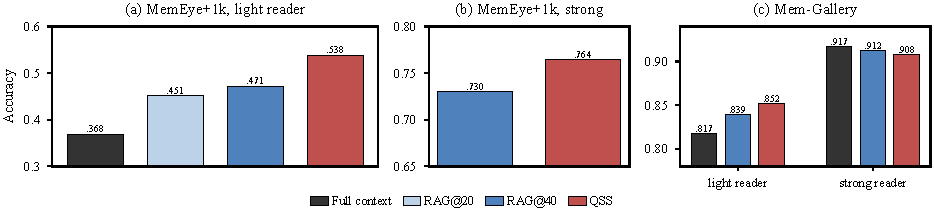
\includegraphics[width=\textwidth]{figures/app_robust.pdf}
\caption{Robustness on MemEye histories enlarged by 1,000 distractor images (MemEye+1k, 371 questions; \qss{} uses a cosine prefilter of 200 rounds) and on Mem-Gallery (903 questions). Full-context reading with the strong reader on MemEye+1k reaches 0.848 on a fixed 100-question subset that is easier than average for retrieval and is not shown.}
\label{fig:app_robust}
\end{figure*}


\section{Selector Models}
\label{app:transfer}

Figure~\ref{fig:app_ablate} compares selector models under the shared prompt. They differ substantially in both full-set recall and the number of selected rounds: \texttt{gemini-3.8-flash} reaches 0.903 with 7.3 rounds, the lightweight Gemini models reach 0.64 to 0.71, and \texttt{gpt-5} and Qwen3-235B-A22B select two to three rounds.

\begin{figure}[t]
\centering
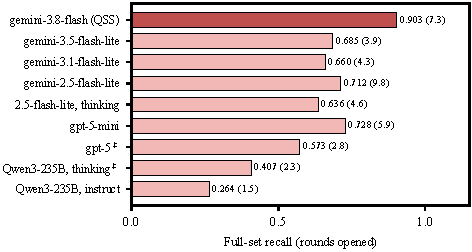
\includegraphics[width=\columnwidth]{figures/app_ablate.pdf}
\caption{Selector models under the shared prompt (MemEye, selection only): full-set recall with the mean number of opened rounds in parentheses. $^\ddagger$A fixed random subset of 150 questions, on which \texttt{gemini-3.8-flash} reaches 0.887 with 7.7 rounds.}
\label{fig:app_ablate}
\end{figure}
\section{Further End-to-End Results}
\label{app:dev}

Table~\ref{tab:e2e} reports further end-to-end results on MemEye, including full-context reading, the annotated evidence, a dynamic cut-off control, and the union of \qss{} with cosine retrieval. Table~\ref{tab:ablation_full} adds the full-set recall of every reading in the ablation of Table~\ref{tab:ablation}.

\begin{table*}[t]
\centering
\small
\begin{tabular}{l|cc|cc|cc}
\toprule
\multirow{2}{*}{\textbf{Reading}} & \multicolumn{2}{c|}{\cellcolor{hME}\textbf{MemEye}} & \multicolumn{2}{c|}{\cellcolor{hML}\textbf{MemLens}} & \multicolumn{2}{c}{\cellcolor{hVM}\textbf{VisualMem}} \\
 & \cellcolor{hME}FSR & \cellcolor{hME}Acc. & \cellcolor{hML}FSR & \cellcolor{hML}Acc. & \cellcolor{hVM}FSR & \cellcolor{hVM}Acc. \\
\midrule
Cosine top-40 (RAG@40) & .914 & .502 & .659 & .466 & .454 & .450 \\
Cosine top-$k$, $k$ = size of the \qss{} set & .527 & .474 & .163 & .416 & .260 & .378 \\
Model ranking, top 8 & .819 & .494 & .466 & .455 & .559 & .537 \\
Model ranking, top $k$, $k$ = size of the \qss{} set & .878 & .523 & .356 & .472 & .555 & .524 \\
\midrule
\qss{}, 100-round pool & .916 & \textbf{.524} & .371 & .483 & .555 & .519 \\
\qss{}, whole index (standard path) & .889 & .518 & .371 & .483 & .793 & .575 \\
Widened path for every question & .887 & .506 & .283 & \textbf{.536} & .766 & .592 \\
\oursrow \vgs{} (visibility gate) & -- & .519 & -- & \textbf{.536} & -- & \textbf{.601} \\
\bottomrule
\end{tabular}
\caption{\textbf{Full ablation with the lightweight reader:} full-set recall (FSR) of the rounds handed to the reader, and accuracy. The model ranking uses the selector and the \qss{} instruction over the same 100-round pool as \qss{} and is cut at 8 rounds or at the size that \qss{} chose. MemLens histories have at most 83 rounds, so the pool is the whole history there. MemEye and VisualMem come from an independent run with regenerated image descriptions.}
\label{tab:ablation_full}
\end{table*}


\begin{table*}[t]
\centering
\small
\resizebox{\textwidth}{!}{%
\begin{tabular}{llrcccr}
\toprule
\rowcolor{hHead} Reader & Method & Rounds & Accuracy & $\Delta$ vs.\ RAG@40 & $\Delta$ vs.\ FC & \$ / 1k q \\
\midrule
\multirow{6}{*}{\shortstack[l]{2.5-flash-lite\\(no thinking)}}
 & Full context (FC) & 126.5 & 0.495 & $+0.007$ & -- & 0.37 \\
 & RAG@40 & 38.7 & 0.488 & -- & $-0.007$ & 0.86 \\
 & Annotated evidence & 2.8 & 0.539 & $+0.051$ & $+0.044$ & 0.17 \\
 & \qss{} & 7.3 & \textbf{0.541} & $+0.053$ $[+0.009, +0.098]$ & $+0.046$ $[+0.001, +0.092]$ & 6.73 \\
 & Dynamic cut-off control & 4.8 & 0.509 & $+0.021$ $[-0.022, +0.064]$ & $+0.013$ & 10.63 \\
 & Union of \qss{} and cosine top-20 & 22.4 & 0.472 & $-0.015$ & $-0.023$ & 7.12 \\
\midrule
\multirow{3}{*}{\shortstack[l]{2.5-flash-lite\\(thinking 1,024)}}
 & Full context (FC) & 126.5 & 0.571 & $+0.019$ & -- & 0.67 \\
 & RAG@40 & 38.7 & 0.552 & -- & $-0.019$ & 1.12 \\
 & \qss{} & 7.3 & \textbf{0.597} & $+0.045$ $[+0.003, +0.086]$ & $+0.026$ $[-0.019, +0.073]$ & 6.97 \\
\midrule
\multirow{7}{*}{3.8-flash}
 & Full context (FC) & 126.5 & \textbf{0.819} & $+0.079$ & -- & 8.97 \\
 & RAG@40 & 38.7 & 0.741 & -- & $-0.079$ & 10.00 \\
 & Annotated evidence & 2.8 & 0.746 & $+0.005$ & $-0.073$ & 2.76 \\
 & \qss{} & 7.3 & 0.761 & $+0.020$ $[-0.014, +0.055]$ & $-0.059$ & 10.27 \\
 & \qss{}, index as context & 7.3 & 0.796 & $+0.055$ $[+0.021, +0.089]$ & $-0.024$ $[-0.050, +0.002]$ & 15.70 \\
 & Dynamic cut-off control & 4.8 & 0.759 & $+0.018$ $[-0.020, +0.055]$ & $-0.061$ & 13.50 \\
 & Union of \qss{} and cosine top-40 & 39.7 & 0.771 & $+0.030$ $[-0.003, +0.063]$ & $-0.049$ & 16.42 \\
\bottomrule
\end{tabular}}
\caption{\textbf{End-to-end results on MemEye.} $\Delta$ columns give paired differences with 95\% question-level bootstrap intervals. Cost is the measured spend per 1k questions over all calls except the judge, without a context cache.}
\label{tab:e2e}
\end{table*}
\section{Visibility Analyses}
\label{app:vis}

\paragraph{Gold rounds of MemLens.} MemLens annotates answer sessions and flags the user turns that state the evidence; the evidence images usually appear in a different turn of the same session than the flagged text. We define the gold rounds of a question as the rounds of its answer sessions that contain a flagged turn or an evidence image (5.9 per question; 4.1 with an image).

\paragraph{Masking.} Figure~\ref{fig:vis}a,b replaces every content word of the question by a placeholder in the index lines of all rounds, while the reader still sees the raw rounds. On MemEye (lightweight reader with thinking), the selector opens 8.5 instead of 7.3 rounds, full-set recall changes by $-0.089$ $[-0.124, -0.054]$, and accuracy by $-0.086$ $[-0.127, -0.045]$. On MemLens (test split, regenerated image descriptions), masking every question word changes full-set recall by $+0.032$ $[+0.006, +0.058]$ and accuracy by $-0.006$ $[-0.032, +0.019]$; on 150 random VisualMem questions, by $0.000$ $[-0.060, +0.060]$ and $-0.007$ $[-0.067, +0.053]$, whereas removing the image descriptions from the index lines changes them by $-0.340$ $[-0.427, -0.253]$ and $-0.093$ $[-0.153, -0.040]$. On MemEye, an index without image descriptions keeps full-set recall at 0.906 but opens 12.3 instead of 7.3 rounds.

\paragraph{Gold definitions.} Figure~\ref{fig:app_gold} recomputes full-set recall on MemLens under alternative gold definitions; the advantage of \qss{} over cosine retrieval of the same size holds under each of them, and 600-character lines raise recall on evidence turns but lower it on evidence images. The derived gold can omit context from the answer sessions that a reader uses.

\begin{figure}[t]
\centering
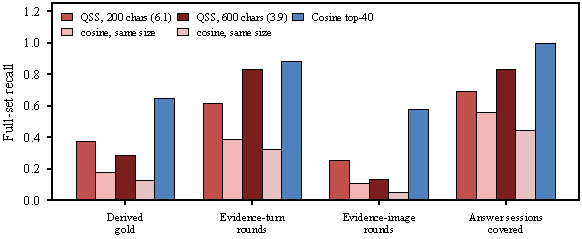
\includegraphics[width=\columnwidth]{figures/app_gold.pdf}
\caption{Full-set recall on MemLens-32k (699 questions) under alternative gold definitions; ``cosine, same size'' opens as many rounds as the selector to its left.}
\label{fig:app_gold}
\end{figure}

\paragraph{Routing policies.} Table~\ref{tab:gate} compares the gate with fixed readings and simple routing rules. Across all 699 MemLens questions, $\hat v(q)$ and the oracle visibility of Eq.~\ref{eq:vis} have means of 0.427 and 0.430 and a Spearman correlation of 0.48. Within a benchmark, $\hat v(q)$ ranks the questions that gain from the widened path only weakly (AUC 0.46 to 0.61).

\begin{table*}[t]
\centering
\small
\begin{tabular}{l|ccc|cc}
\toprule
\rowcolor{hHead} & \multicolumn{3}{c|}{\textbf{Lightweight reader}} & \multicolumn{2}{c}{\textbf{Strong reader}} \\
\rowcolor{hHead} \textbf{Policy} & MemEye & MemLens & VisualMem & MemEye & MemLens \\
\midrule
Standard path for every question & 0.518 & 0.483 & 0.575 & 0.803 & 0.618 \\
Widened path for every question & 0.506 & 0.536 & 0.592 & 0.749 & 0.689 \\
Gate on message length & 0.501 & 0.530 & 0.593 & 0.800 & 0.687 \\
Random routing, same share & 0.517 & 0.530 & 0.585 & 0.802 & 0.680 \\
\oursrow \vgs{} gate ($\hat v(q)\ge0.7$) & 0.519 & 0.536 & 0.601 & 0.797 & 0.687 \\
\midrule
Per-question oracle & 0.612 & 0.597 & 0.655 & 0.842 & 0.734 \\
AUC of $\hat v(q)$ & 0.46 & 0.55 & 0.61 & -- & -- \\
\bottomrule
\end{tabular}
\caption{\textbf{Routing policies.} Each cell is the accuracy when every question takes the given path or when a rule routes it; the widened path of the strong reader is top-40 retrieval. The message-length gate widens a question when the user messages of its ten most similar rounds average at least 165 characters, a threshold chosen on MemEye and the remaining MemLens questions as for $\tau$. AUC: how well $-\hat v(q)$ ranks the questions on which the widened path scores higher than the standard path above those on which it scores lower. MemEye and VisualMem with the lightweight reader use the run of Table~\ref{tab:ablation}.}
\label{tab:gate}
\end{table*}

\section{Cost and Deployment}
\label{app:cost}

\paragraph{Cost model.} Costs use list prices per million tokens: \texttt{gemini-3.8-flash} \$0.75 input, \$0.075 cached input, \$3.75 output (including thinking); \texttt{gemini-2.5-flash-lite} \$0.10, \$0.01, and \$0.40; \texttt{gemini-embedding-2} \$0.20 for text and \$0.45 for images. Measured costs use the cached-token counts reported by the API and include the creation and storage of explicit caches, amortized over the questions asked of each history. Writing the index costs one caption per image (about \$0.001 for a short caption with \texttt{gemini-3.8-flash}) and one embedding per round.

\begin{figure}[t]
\centering
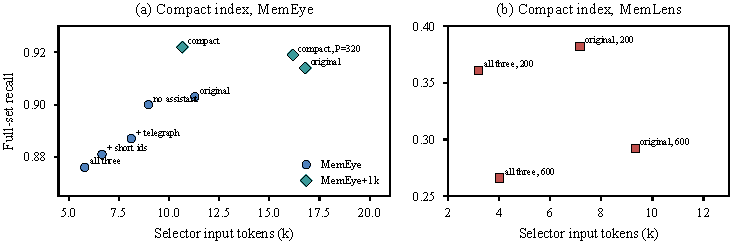
\includegraphics[width=\columnwidth]{figures/app_compact.pdf}
\caption{Selection with compact indexes (\texttt{gemini-3.8-flash} selector): ``no assistant'' drops the assistant snippet, ``short ids'' lists rounds by positional identifiers under one header per session, ``telegraph'' removes function words from the user text before truncation, and ``compact'' combines no assistant and telegraph; MemEye+1k uses a cosine prefilter of $P$ rounds.}
\label{fig:app_compact}
\end{figure}
\paragraph{Compact index.}
\label{app:compact}
Figure~\ref{fig:app_compact} reports the selection results behind the compact index. Dropping the assistant snippet removes about a fifth of the input with almost no loss of full-set recall (0.900 against 0.903 on MemEye), short identifiers remove another fifth at a small loss, and together the three rules let 600 characters of a long MemLens message fit into fewer tokens than the original 200-character lines (4,026 against 7,166 tokens). On the MemEye questions with at least four gold rounds, full-set recall falls from 0.872 to 0.791 with all three rules.

\paragraph{Deployment variants.} Table~\ref{tab:p6} collects the cost-aware variants: an explicit cache of the original and of the compact index on persistent histories, and budget controls such as top-40 retrieval with thinking.

\begin{table*}[t]
\centering
\small
\resizebox{\textwidth}{!}{%
\begin{tabular}{lllccr}
\toprule
\rowcolor{hHead} Data & Reader & Method & Accuracy & $\Delta$ vs.\ RAG@40 & \$ / 1k q \\
\midrule
\multirow{6}{*}{MemEye} & \multirow{4}{*}{2.5-flash-lite}
 & RAG@40 & 0.488 & -- & 0.86 \\
 & & RAG@40 with thinking & 0.552 & $+0.064$ $[+0.011, +0.117]$ & 1.12 \\
 & & \qss{} with thinking, uncached index & 0.597 & $+0.109$ $[+0.055, +0.166]$ & 6.97 \\
 & & \qss{} with thinking, cached index & \textbf{0.590} & $+0.102$ $[+0.049, +0.158]$ & 2.58 \\
\cmidrule{2-6}
 & \multirow{2}{*}{3.8-flash}
 & RAG@40 & 0.749 & -- & 9.78 \\
 & & \qss{} with index, cached index & \textbf{0.800} & $+0.051$ $[+0.015, +0.088]$ & 7.04 \\
\midrule
\multirow{2}{*}{Mem-Gallery} & \multirow{2}{*}{3.8-flash}
 & RAG@40 & 0.912 & -- & 5.70 \\
 & & \qss{} with index, cached index & 0.910 & $-0.001$ $[-0.012, +0.009]$ & 5.97 \\
\midrule
\multirow{4}{*}{MemLens-64k} & \multirow{2}{*}{2.5-flash-lite}
 & RAG@40 & 0.468 & -- & 1.45 \\
 & & VGS & \textbf{0.524} & $+0.056$ $[+0.015, +0.097]$ & 14.81 \\
\cmidrule{2-6}
 & \multirow{2}{*}{3.8-flash}
 & RAG@40 & 0.655 & -- & 12.75 \\
 & & RAG@40 with abstention fallback & \textbf{0.697} & $+0.043$ $[+0.026, +0.062]$ & 12.85 \\
\midrule
\multicolumn{6}{l}{\emph{With a compact index}} \\
MemEye & 2.5-flash-lite & \qss{} with thinking, cached & 0.589 & $+0.101$ $[+0.046, +0.156]$ & 1.83 \\
MemEye & 3.8-flash & \qss{} with index, cached & \textbf{0.803} & $+0.053$ $[+0.020, +0.088]$ & 6.27 \\
MemLens-64k & 2.5-flash-lite & VGS & \textbf{0.528} & $+0.060$ $[+0.021, +0.099]$ & 7.03 \\
\bottomrule
\end{tabular}}
\caption{\textbf{Deployment variants.} MemEye and Mem-Gallery are persistent histories, so the index can be served from an explicit context cache (costs include cache creation and storage); MemLens has one haystack per question, so nothing is cached. $\Delta$ gives paired differences from RAG@40 with the same reader and 95\% bootstrap intervals.}
\label{tab:p6}
\end{table*}
\section{Reproducibility}
\label{app:repro}

All code, per-question outputs (retrieved rounds, prediction, judge score and rationale, token usage), and logs are in the project repository, whose README maps every table and figure to the script that recomputes it from the stored outputs without API calls. Re-running a condition issues new model calls, whose outputs, such as image captions, can differ slightly from the stored ones. All subsets, samples, and random orders are fixed by stored identifiers and seeds.

\section{VisualMem Details}
\label{app:visualmem}

\paragraph{Data.} VisualMem~\citep{nguyen2026personalvisual} provides ten personas, each with about 171 dated events whose conversations contain one shared image, and 696 multiple-choice questions with four options; 631 have text options and 65 have image options, and six attach a query image. A question asks about a fact that the authors placed only in the image of an earlier event, for example the equipment that stands on the left side of a balcony, or about a recurring entity such as a pet. We treat each event as a session and each user turn with the following assistant turn as a round, ask all questions after the whole history, and take the image rounds of the event that a question belongs to as its gold rounds. Images are downscaled to 1,024 pixels on the longer side for all methods, and scoring compares the first option letter of the answer with the gold letter.

\paragraph{Visual dependence.} Figure~\ref{fig:app_vm}a removes all visual information (images and their descriptions). With the annotated evidence, accuracy falls from 0.609 to 0.297, close to the chance level of 0.25, so the questions depend on the images. Top-40 retrieval keeps 91\% of its accuracy without visual information, because it contains the evidence round for only 45.4\% of the questions.

\begin{figure}[t]
\centering
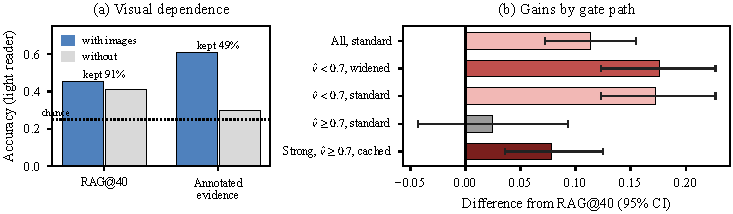
\includegraphics[width=\columnwidth]{figures/app_visualmem.pdf}
\caption{VisualMem. (a)~Accuracy with and without visual information, lightweight reader (696 questions). (b)~Gains over RAG@40 by gate path with 95\% bootstrap intervals (415 questions below the threshold, 281 above it).}
\label{fig:app_vm}
\end{figure}

\paragraph{Results by path.} Figure~\ref{fig:app_vm}b splits the VisualMem results at the gate. The estimated visibility has a mean of 0.655, and the oracle visibility of Eq.~\ref{eq:vis} has a mean of 0.769. Cache creation and storage add \$3.69 per 1,000 questions to the lightweight reader and \$3.60 to the strong reader; both are included in Table~\ref{tab:main}.



\section{Results on the Full Question Sets}
\label{app:fulltest}

Table~\ref{tab:fulltest} reports \vgs{} against top-40 retrieval on the full question sets, including the 466-question MemLens test split at the 32k and 64k history lengths.

\begin{table}[t]
\centering
\small
\resizebox{\columnwidth}{!}{%
\begin{tabular}{llccr}
\toprule
\rowcolor{hHead} Data & Method & Acc. & $\Delta$ vs.\ RAG@40 & \$/1k \\
\midrule
\multicolumn{5}{l}{\textit{Lightweight reader (\texttt{gemini-2.5-flash-lite})}} \\
\multirow{2}{*}{MemEye} & RAG@40 & 0.488 & -- & 0.86 \\
& \vgs{} & \textbf{0.541} & $+0.053$ $[+0.009, +0.098]$ & 6.76 \\
\multirow{2}{*}{MemLens-32k} & RAG@40 & 0.466 & -- & 1.73 \\
& \vgs{} & \textbf{0.536} & $+0.071$ $[+0.032, +0.109]$ & 8.63 \\
\multirow{3}{*}{MemLens-64k} & RAG@40 & 0.468 & -- & 1.45 \\
& \vgs{} & 0.524 & $+0.056$ $[+0.015, +0.097]$ & 14.81 \\
& \vgs{}, compact index & \textbf{0.528} & $+0.060$ $[+0.021, +0.099]$ & 7.03 \\
\multirow{2}{*}{VisualMem} & RAG@40 & 0.454 & -- & 0.96 \\
& \vgs{}, cached index & \textbf{0.569} & $+0.115$ $[+0.075, +0.157]$ & 13.70 \\
\midrule
\multicolumn{5}{l}{\textit{Strong reader (\texttt{gemini-3.8-flash})}} \\
\multirow{2}{*}{MemEye} & RAG@40 & 0.749 & -- & 9.78 \\
& \vgs{}, cached index & \textbf{0.797} & $+0.048$ $[+0.015, +0.082]$ & 6.21 \\
\multirow{2}{*}{MemLens-32k} & RAG@40 & \textbf{0.689} & -- & 14.74 \\
& \vgs{} & 0.687 & $-0.002$ $[-0.017, +0.013]$ & 14.24 \\
\multirow{2}{*}{MemLens-64k} & RAG@40 & \textbf{0.655} & -- & 12.75 \\
& \vgs{} & 0.648 & $-0.006$ $[-0.026, +0.013]$ & 13.32 \\
\multirow{2}{*}{VisualMem} & RAG@40 & 0.812 & -- & 8.79 \\
& \vgs{}, cached index & \textbf{0.843} & $+0.032$ $[+0.014, +0.050]$ & 16.80 \\
\bottomrule
\end{tabular}}
\caption{\textbf{\vgs{} on the full question sets.} Accuracy and measured cost per 1,000 questions. $\Delta$ is the paired difference from RAG@40 with the same reader and a 95\% bootstrap interval. Strong-reader costs on MemEye use the compact cached index; cached costs include cache creation and storage.}
\label{tab:fulltest}
\end{table}

\section{Standard Metrics and Latency}
\label{app:latency}

\begin{table*}[t]
\centering
\footnotesize
\setlength{\tabcolsep}{2.4pt}
\begin{tabular}[t]{l|cc|cc}
\toprule
\rowcolor{hHead} & \multicolumn{2}{c|}{\textbf{Token F1}} & \multicolumn{2}{c}{\textbf{BLEU-1}} \\
\rowcolor{hHead} \textbf{Method} & MemEye & MemLens & MemEye & MemLens \\
\midrule
RAG@40 & .304 / .508 & .467 / .639 & .259 / \textbf{.448} & .454 / .616 \\
SimpleMem & .250 / .329 & .346 / .375 & .211 / .290 & .335 / .362 \\
Omni-SimpleMem & .187 / .236 & .378 / .397 & .149 / .201 & .368 / .381 \\
MIRIX & .174 / .202 & .231 / .184 & .142 / .179 & .226 / .180 \\
V-Mem & .294 / .442 & .435 / .561 & .249 / .391 & .420 / .539 \\
MMA & .260 / .380 & .447 / .492 & .214 / .330 & .433 / .466 \\
TeleMem & .246 / .290 & .295 / .157 & .207 / .255 & .285 / .152 \\
\midrule
\oursrow \vgs{} (ours) & \textbf{.351} / \textbf{.511} & \textbf{.496} / \textbf{.662} & \textbf{.301} / .447 & \textbf{.480} / \textbf{.638} \\
\bottomrule
\end{tabular}\hfill
\begin{tabular}[t]{l|ccc|ccc}
\toprule
\rowcolor{hHead} & \multicolumn{3}{c|}{\textbf{Recall@10}} & \multicolumn{3}{c}{\textbf{nDCG@10}} \\
\rowcolor{hHead} \textbf{Method} & ME & ML & VM & ME & ML & VM \\
\midrule
RAG@40 & .774 & .579 & .299 & .667 & .537 & .226 \\
V-Mem & .621 & .583 & .272 & .409 & .452 & .202 \\
MMA & .697 & \textbf{.786} & .355 & .550 & \textbf{.808} & .246 \\
\midrule
\oursrow \vgs{} (ours) & \textbf{.903} & .626 & \textbf{.753} & \textbf{.829} & .723 & \textbf{.656} \\
\bottomrule
\end{tabular}
\caption{\textbf{Standard metrics.} On the question sets of Table~\ref{tab:main}. Left: token F1 and BLEU-1 of the answers (lightweight / strong reader) on the open-ended benchmarks; VisualMem is multiple choice, so its answer metric is the exact match of Table~\ref{tab:main}. Right: Recall@10 and nDCG@10 of the rounds that a method hands to the reader, in its own order, against the gold rounds (\vgs{}: its lightweight-reader path). They apply to the methods that return raw rounds; the other memory systems return rewritten records. Latency is in Table~\ref{tab:latency}.}
\label{tab:std}
\end{table*}


\paragraph{Answer metrics.} Token F1 and BLEU-1 (Table~\ref{tab:std}) follow the LoCoMo evaluation: answers and references are lower-cased, punctuation and articles are removed, and tokens are split on white space; BLEU-1 is the clipped unigram precision with the brevity penalty.

\paragraph{Evidence metrics.} Recall@10 is the fraction of gold evidence rounds among the first ten rounds that a method hands to the reader, in the method's own order (cosine rank for top-40 retrieval, the selector's order for \vgs{}, and the order returned by V-Mem and MMA), and nDCG@10 uses binary relevance. The rounds of V-Mem and MMA come from a re-run of their retrieval; V-Mem indexes regenerated image captions, and its re-run returns the same number of rounds as the main run for 25\%, 57\%, and 50\% of the MemEye, MemLens, and VisualMem questions (MMA: the same number of images for 98\%, 91\%, and 98\%).

\paragraph{Latency.} We measure wall-clock time per question from receiving the question to the reader's answer, with the memory already built, one question at a time, on one machine and network: 30 questions of one MemEye history (120 rounds), 10 MemLens-32k questions with their own histories, and 30 questions of one VisualMem persona (1,013 rounds). Each method runs its own retrieval, including any model calls, followed by the same reader call; the first question of a persistent history is excluded because it creates the context cache. Table~\ref{tab:latency} lists the medians for both readers, the retrieval time of each method, and the construction time per history. About 3\% of the calls of every method stalled until the 240-s client timeout and were retried, so we report medians. Construction uses the default parallelism of each system; for MIRIX, whose agents occasionally stalled and were restarted, it sums the completed additions of sessions.

\begin{table*}[t]
\centering
\small
\setlength{\tabcolsep}{3.2pt}
\begin{tabular}{l|cc|cc|cc|ccc}
\toprule
\rowcolor{hHead} & \multicolumn{2}{c|}{\cellcolor{hME}\textbf{MemEye}} & \multicolumn{2}{c|}{\cellcolor{hML}\textbf{MemLens}} & \multicolumn{2}{c|}{\cellcolor{hVM}\textbf{VisualMem}} & \multicolumn{3}{c}{\textbf{Construction (s per history)}} \\
\rowcolor{hHead} \textbf{Method} & Answer & Retrieval & Answer & Retrieval & Answer & Retrieval & MemEye & MemLens & VisualMem \\
\midrule
RAG@40 & 5.4 / 8.8 & 1.2 & 16.5 / 9.9 & 1.7 & 15.7 / 8.4 & 1.6 & 20.4 & 10.9 & 44.7 \\
SimpleMem & 22.0 / 22.5 & 20.5 & 22.6 / 23.1 & 21.3 & 23.8 / 25.2 & 21.8 & 158 & 38.8 & 808 \\
Omni-SimpleMem & 3.0 / 4.2 & 1.7 & 4.2 / 4.0 & 1.4 & 5.5 / 8.0 & 3.6 & 685 & 172 & 2,701 \\
MIRIX & 5.0 / 6.8 & 3.4 & 5.4 / 6.3 & 3.8 & 4.9 / 8.3 & 3.1 & 1,694 & 868 & 11,738 \\
V-Mem & 3.6 / 5.8 & 0.0 & 2.8 / 6.8 & 0.0 & 2.4 / 5.9 & 0.0 & 0.4 & 0.6 & 5.8 \\
MMA & 2.3 / 4.7 & 0.0 & 5.7 / 4.7 & 0.4 & 4.1 / 7.7 & 1.4 & 632 & 21.1 & 276 \\
TeleMem & 2.0 / 3.3 & 0.9 & 3.9 / 3.8 & 1.2 & 1.8 / 3.0 & 0.8 & 86.3 & 38.2 & 507 \\
\midrule
\oursrow \vgs{} (ours) & 6.3 / 10.7 & 4.1 & 14.1 / 9.9 & 6.6 & 12.7 / 11.2 & 5.5 & 20.4 & 10.9 & 44.7 \\
\bottomrule
\end{tabular}
\caption{\textbf{Latency and construction time.} On the latency samples (Appendix~\ref{app:latency}): median seconds per question with the lightweight / strong reader, the median retrieval time of each method (including its model calls; for \vgs{}, the selection call), and the memory construction time per history (seconds; MemEye: one history of 120 rounds, MemLens: median over the 10 histories, VisualMem: one persona of 1,013 rounds).}
\label{tab:latency}
\end{table*}


\section{External Memory Systems}
\label{app:baselines}

Table~\ref{tab:systems} summarizes the six systems. Every system builds one memory per history from the same rounds, in chronological order and with dates, and the same one-sentence image descriptions as our index; the multimodal systems also receive the raw images. Memory construction uses \texttt{gemini-3.8-flash} with low thinking unless the table lists another model, and \texttt{gemini-embedding-2} serves as the joint text-image embedding wherever a system embeds images. Each system retrieves with its own method from the full question text, and the reader receives the retrieved memory, with any images that the system returns, under the same system prompt and answer format as all other methods, followed by the same judges. Costs include memory construction, amortized over the questions of each benchmark. On MemLens, each question has its own history, so the systems run on 150 test questions stratified by type; MIRIX did not finish building the memories of 2 MemEye and 10 MemLens histories, so its results use the other 269 and 140 questions.

\begin{table*}[t]
\centering
\small
\setlength{\tabcolsep}{3.4pt}
\begin{tabular}{l|p{4.1cm}|p{3.6cm}|p{2.7cm}|p{3.3cm}}
\toprule
\rowcolor{hHead} \textbf{System} & \textbf{Memory written at ingestion} & \textbf{Retrieval (budget)} & \textbf{Other models} & \textbf{Adaptation} \\
\midrule
SimpleMem (0.3.0) & factual statements from windows of 40 turns, with resolved references and times & planning, reflection, hybrid search & -- & punctuation removed from keyword queries \\
Omni-SimpleMem (0.3.0) & multimodal atomic units, knowledge graph; images as on-demand units & hybrid search, graph expansion (20 units) & unit summaries: 2.5-flash-lite & no modality filter for questions about images \\
MIRIX (0.1.5) & typed memories written by six agents & memory extraction for the question & \texttt{gemini-2.5-flash} & images passed as JPEG copies \\
TeleMem (1.10.1) & one memory per message, for the user profile and for events & top 30 per scope & extraction: 2.5-flash-lite & English extraction prompts \\
V-Mem & raw user, assistant, and image units of every round & modality routing (12 rounds and neighbours) & anchors: 2.5-flash-lite & -- \\
MMA & raw turns with a confidence score & similarity $\times$ confidence (10 turns) & -- & -- \\
\bottomrule
\end{tabular}
\caption{\textbf{External memory systems.} Released code and default settings; MMA as implemented in the official MemEye evaluation framework. ``Other models'' lists roles that do not use \texttt{gemini-3.8-flash}; ``Adaptation'' lists the changes needed to run each release on our data.}
\label{tab:systems}
\end{table*}

\paragraph{Paired differences.} Figure~\ref{fig:app_baselines} shows the paired differences of every method from top-40 retrieval with bootstrap intervals.

\begin{figure*}[t]
\centering
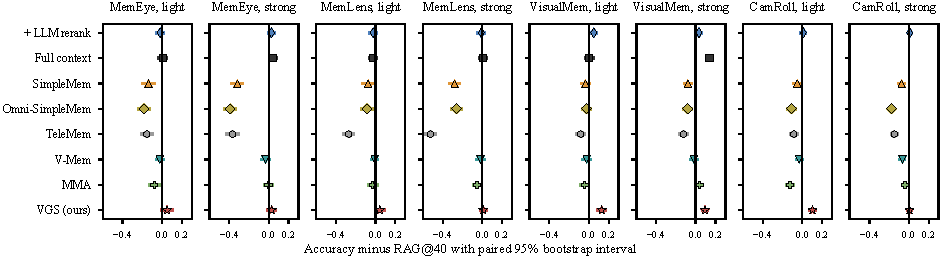
\includegraphics[width=\textwidth]{figures/app_baselines.pdf}
\caption{Paired difference of every method from RAG@40 with 95\% bootstrap intervals on the question sets of Table~\ref{tab:main}.}
\label{fig:app_baselines}
\end{figure*}
